\subsection{What is OFDM}

The Orthogonal Frequency Division Multiplexing (OFDM) is a multicarrier modulation strategy. In counterpoint with a single carrier modulation system of which the data modulate a carrier with single frequency, the OFDM strategy uses multiples carriers to modulate the data segmented in as many channels as subcarriers available. 

The catch with the OFDM is that the carriers obey the principle of orthogonality, with each subarrier closely spaced, allowing each data channel bandwidth to superposed between themselves, but without loss of information, different that would happen in a Frequency Division Multiplex (FDM) channel. Therefore the major data stream is segmented into minor flows with lower rate and large symbol time.

\subsection{OFDM transmitter with IFFT}

For sake of simplicity an OFDM transmitter can be split in some sections, so each transformation in the original sequence of bits and its effects in the output signal becomes clearly. The steps followed to generate a OFDM signal is as follows:

\begin{itemize}
    \item Convert original frame from series to parallel representation (S/P);
    \item Map blocks of bits in a M-QAM constellation;
    \item Ensure the conjugate symmetry property of DFT upon M-QAM sequence of constellation points;
    \item Modulation with IDFT (IFFT for higher efficiency);
    \item Further insertion of the cyclic prefix.
\end{itemize}

\subsubsection{Serial-to-parallel conversion}

The original serial bit stream that is normally modulated with a single carrier is split in a serial-to-parallel buffer with frames of size $N_f$ bits.  Soon after each frame is parsed into $N_c$ blocks, so each block of bits can be modulated in a multi carrier fashion and each block representing a channel. Each individual block can be encoded as the designer wishes. The equation \ref{eq:bit_sum} translates the i-th block has $b_i$ bits, and when summed all bits, the frame size is achieved:

\begin{equation} \label{eq:bit_sum}
    \sum_{i=1}^{N_c} b_i = N_f
\end{equation}

It is important to disclosure that this paper will work with sequences of positive non-null index (in the majority of time), so each sequence can be represented conveniently in a software simulation.

\subsubsection{Constellation mapping}

The $N_c$ blocks must have its bits modulated with a M-QAM modulation, so each M-QAM symbol can be mapped into a constellation map. A constellation point is represented by a complex number with an in-phase value (real) and a quadrature value (imaginary). Therefore, each channel represented by a different M-QAM constellation with same symbol time of $1/T$ will employ $M = 2^{b_i}$ signal points. Each constellation point in the k-th channel can be represented by $X_k$, where $k = 1,..,N_c$. 

\subsubsection{Symmetry of DFT}

The $\{X_k\}$ sequence is read as the DFT over an OFDM time signal. So applying the IDFT over the sequence $\{X_k\}$ it is expected to obtain the OFDM time signal to be transmitted. Sure the IDFT can be applied in the sequence $\{X_k\}$ as it is, but it will generate a complex time series that needs an additional modulation step via a phase and quadrature modulator. 

The solution to avoid the use of such modulator is transforming the sequence $\{X_k\}$ in such way that its magnitude is an even function of frequency and its phase response is an odd function, therefore ensuring the conjugate symmetry property of the DFT.

This can be done extending the sequence $\{X_k\}$ of size $N_c$ into a sequence of size $2N_c$ and inserting into this upper half of the sequence the complex conjugate of the original sequence (lower half). The new points of the sequence can be populated as:

\begin{equation} \label{eq:symmetry}
    X_{2N_c-k}=X_k^*, \; \; k = 2,...,2N_c
\end{equation}

The first point of the original $\{X_k\}$ is divided in two real points and distributed in the beginning of the sequence ($X_1= \Re(X_1)$) and at the middle of the sequence ($X_{N_c} = \Im(X_1)$).

\subsubsection{Multicarrier modulation with IFFT}

Once the new sequence $\{X_k\}$ with length $2N_c$ is obtained and respects the conjugate symmetry properties, each point can be modulated by a different subcarrier over a symbol period. This is made with the help of the IDFT, but to achieve high efficiency, the IFFT algorithm is largely used. 

As we can see in the equation \ref{eq:idft}, the variable $x_n$ represent a sample of an OFDM symbol and the full sequence $\{x_n, \, 0 \leq n \leq 2N_c-1\}$ nonetheless represents an OFDM symbol. It is important to see that each $X_k$ point is modulated by a complex exponential whose frequency is dependent of $k$, ensuring that each individual channel is modulated by a different carrier. Once $n$ varies over $n = 0,1,...,2N_c-1$, we can see that the sequence $\{X_k\}$ is maintained until, at least, one period of each subcarrier is achieved, concluding the synthesis of the sequence $\{x_n\}$ of length $2N_c$ that represents an OFDM symbol of which contains $N_c$ different M-QAM symbols.

\begin{equation} \label{eq:idft}
    x_n = \frac{1}{\sqrt{N}} \sum_{k=1}^{2N_c} X_k e^{j2\pi n(k-1)/(2N_c)}, \; \; n = 0,1,...,2N_c-1
\end{equation}

\subsubsection{Cyclic prefix}

Considering a dispersive channel with impulse response $c(t)$, and $n(t)$ some additive noise, the continuous OFDM signal in the medium will suffer the following distortion:

\begin{equation}
    r(t) = x(t) \ast c(t) + n(t)
\end{equation}

If the designer chooses the frequency bandwidth of each subchannel to be $\Delta f$ as small as possible, the symbol duration $T=1/\Delta f$ will be large if we compare with the channel dispersion with $\nu$ samples. A solution to avoid ISI is to add a guard band of duration $\nu T/(2N_c)$ so the effect of the channel in one symbol is isolated from another.

To observe the effect of the channel dispersion, we have simulated a transmission of a NRZ polar signal in two different hypothetical channel scenarios. The results are shown in the figure \ref{fig:channel_influence}. Both channel are modulated by a first order transfer function for the sake of simplicity. The first channel has a settling time of 4 seconds ($1/(s+1)$) and the second has a settling time of 0.4 seconds ($10/(s+10)$). The symbol duration of the NRZ signal was choose to be 1 second, so as we can see in the figure \ref{fig:channel_influence}, the dynamics of the channel 1 exerts high influence in all the symbol time and does not have time to settle its response before the next symbol, so it distort the receive signal in the point to harm the quality of the signal. Therefore the channel 2 that has a settling time lower than the symbol time, having a minor influence in the symbols and restricting its influence inside a symbol period.

\begin{figure}[h]
\begin{center}
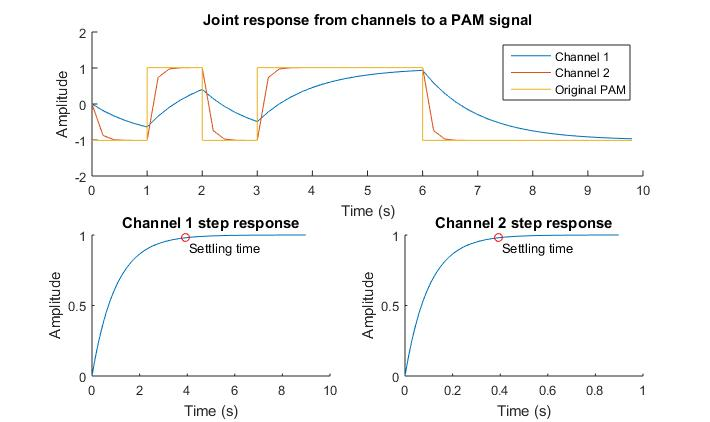
\includegraphics[width=8.5cm]{images/channel_influence.jpg}
\caption{Different channel influence in a transmission. Source: own.}
\label{fig:channel_influence} 
\end{center}
\end{figure}

An alternative way to avoid ISI in the OFDM signal is to append a cyclic prefix in each block of $2N_c$ samples $\{X_0,...,X_{2N_c-1}\}$. The cyclic prefix is a sequence extract from the previous block of samples that consists in the $\nu$ last samples of the block $\{X_{2N_c-\nu},...,X_{2N_c-1}\}$ and then added to the beginning of the sequence. 

Once $\nu$ is the number of samples that the channel dispersion lasts the final sequence have a length of $2N_c+\nu$ samples and the cyclic prefix will work as a time guard band against ISI. Further in reception these samples are discarded, once only the original sequence matters to extract information.

There is also another way to overcome the channel response, which its estimation and compensation with equalizers. But for this, there is a need to measure the channel response of which can be accomplished by transmitting either a known modulated sequence on each of the subcarriers or transmitting the unmodulated subcarriers.
